
\chapter{Data}
\section{GRACE and GRACE-FO}
\subsection{Spherical harmonics}
The variations in the gravity field impacts on both GRACE satellites at different times, such deviations cause a change in the inter-satellite range, which is measured with very high accuracy from the K-band measurement unit. The measured inter-satellite range can be transformed into changes in teh Earth's gravity field, which is described with the Stokes coefficients $\tilde{C}_{lm}$ and $\tilde{S}_{lm}$.\\\\
There is only one Earth gravity field and all centers start off with identical GRACE Level-1 observations, but deriving month-to-month gravity field variations from GRACE observations requires a complex inversion of relative ranging observations between the two formation-flying GRACE spacecraft, in combination with precise orbit determination via GPS and various corrections for spacecraft accelerations not related to gravity changes. Many parameter choices and solution strategies are possible, and have been explored by different data centers. In this thesis the solutions from JPL, CSR, GFZ and ITSG are used, which allows the calculation of gravity filed and equivalent water height anomaly. \autoref{shmethod} shows the method of estimating TWS from GRACE spherical harmonics: 
\begin{equation}
h_{W}(\theta,\lambda;t) = \frac{R \rho_{ave}}{3\rho_{W}} \sum_{l=0}^{\infty} \frac{2l+1}{1+k_{l}} \sum_{m=0}^{l} \tilde{P}_{lm} (\cos \theta) (\Delta \tilde{C} \cos m \lambda + \Delta \tilde{S} \sin m \lambda)
\end{equation}
\subsection{Mass concentration}
Spherical harmonics have been well studied and widely used in satellite geodesy for several decades, based on the computational efficiency of the parameterization, and because the satellite sensitivity is dependent on the spatial wavelength of the mass variations which is implicit in the harmonic basis function. However, unconstrained harmonic solutions from GRACE have typically suffered from poor observability of east-west gradients, resulting in the so-called "stripes" that are conventionally removed via empirical smooting and-or "destriping" algorithms. Although quite effective, especially for larger spatial scales,the destriping also removes some real geophysical signal along with the stripes,and the size shape, and orientation of the signals strongly affect the effectiveness of destriping.\cite{watkins2015improved} \\\\
Thus, to confirm the reliability of spherical harmonic, another common function would be be taken into consideration to estimate mass flux from GRACE, which is called mass concentration(mascon). Each mass tile are defined as a finite truncated spherical harmonic representation up to degree and order 120, which are in turn related to the range-rate observation via their partial derivatives. The size of each tile is aproximately $1^{\circ}$ equatorial longitudinal distance. The mass anomaly for each of the mass tile is estimated using the KBR range-rate observations and the associated spherical harmonic partial derivatives and the singular estimation process is stabilized using Tikhonov regularization solutions with time-variable regularization matrix. \cite{save2016high}. \\\\
This mascon solutions have no stripe errors and capture all the signals ovserved by GRACE within the measurement noise level. The solutions are not tailored for specific applications and are global in nature.\cite{save2016high} 
\begin{figure}[htbp]
	\centering
	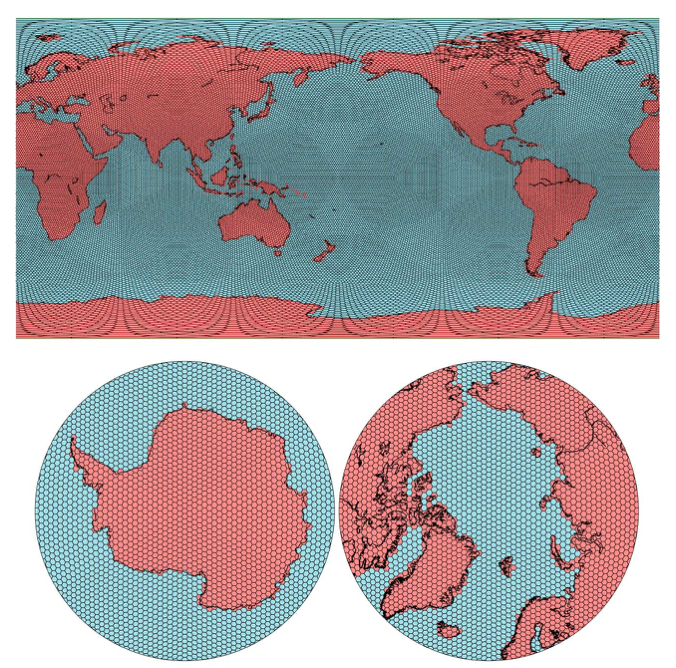
\includegraphics[width=0.5\textwidth]{mascon} % Datei in "bilder/" bei LaTeX: eps, bei PDFLaTeX: jpg (o.ä.) 
	\caption{The distribution of 40,962 geodesic grid tiles over the Earth used as a basis function for estimation of mass
		anomalies from GRACE for CSR mascon solutions. (top) Global view, (bottom left) South Pole view, and (bottom right) North Pole view \cite{save2016high}} 
	\label{fig:mascon}
\end{figure}
In this thesis the mascon solution from CSR are compared with the results from spherical harmonic solutions.
\newpage
\section{Precipitation}
Gauge observations are typically used to measure precipitation directly at the Earth's surface \cite{kidd2001satellite}. Various large-scale climate data sets at different spatiotemporal scales have been developed from station (in situ) observations. These different types of precipitation data product have proved useful across a wide range of fields of research \cite{sun2018review}.
In this thesis the precipitation data from 9 data resources are gathered and processed (\autoref{tab:pre}). The methods dealing with these data sets will be discussed later:
\begin{table}[htbp]\centering 
	\begin{tabular}{|l|l|l|l|l|}
		\hline
		\textbf{Dataset}      & \textbf{Timespan}       & \textbf{Temporal Resolution} & \textbf{Spatial Resolution} & \textbf{Spatial Coverage} \\ \hline
		PREC/L       & 1948 - present & Monthly             & $0.5^{\circ} \times 0.5^{\circ}$          & Global           \\ \hline
		CPC          & 1979 - present & Monthly , Daily    & $0.5^{\circ} \times 0.5^{\circ}$          & Global           \\ \hline
		GPCP         & 1979 - present & Monthly             & $2.5^{\circ} \times 2.5^{\circ}$          & Global           \\ \hline
		CMAP         & 1979 - present & Monthly             & $2.5^{\circ} \times 2.5^{\circ}$          & Global           \\ \hline
		PERSIANN-CDR & 1983 - present & Monthly , Daily    & $0.25^{\circ} \times 0.25^{\circ}$        & $60S^{\circ} - 60N^{\circ}$      \\ \hline
		NCEP1        & 1948 - present & Monthly , Daily    & $2.5^{\circ} \times 2.5^{\circ}$          & Global           \\ \hline
		NCEP2        & 1979 - present & Monthly , Daily    & $1.875^{\circ} \times 1.875^{\circ}$      & Global           \\ \hline
		ERA5         & 1979 - present & Monthly             & $31\ut{km} \times 31\ut{km}$        & Global           \\ \hline
		MERRA-2      & 1980- present  & Monthly , Daily    & $0.5^{\circ} \times 0.625^{\circ}$        & Global           \\ \hline
	\end{tabular}
	\caption{precipitation datasets}
	\label{tab:pre}
\end{table}
\paragraph{Precipitation reconstruction over land (PREC/L)}
PREC/L if provided from National Oceanic and Atmospheric Administration (NOAA).It is derived from gauge observations from over 17 000 stations collected in the Global Historical Climatology Network(GNCN), and the Climate Anomaly Monitoring System(CAMS) datasets. By using OI analysis procedure, the monthly gridded analyses of precipitation over the global land area since 1948 are presented. The mean distribution and annual cycle of precipitation observed in the PREC/L showed good agreement with those in several published gauge-based datasets. \cite{chen2002global}
\paragraph{CPC unified gauge-based analysis of global daily precipitation}
This dataset is provided from Climate Prediction Center(CPC). A gauge-based analysis of daily precipitation has been constructed over the global land areas. Gauge reports from over 30 000 stations are collected from multiple sources including GTS, COOP, and other national and international agencies. Quality control is performed through comparisons with historical records and independent information from measurements at nearby stations, concurrent radar / satellite observations, as well as numerical model forecasts. Quality controlled station reports are then interpolated to create analyzed fields of daily precipitation with consideration of orographic effects \cite{xie2007gauge}. The daily analysis is constructed on a 0.125 degree lat/lon grid over the entire global land areas, and released on a 0.5 degree lat/lon grid over the global domain for a period from 1979 to the present.\cite{xie2010cpc} This dataset has two components: (a) the "retrospective version" which uses 30K stations and spans 1979-2005 and (b) the "real-time version" which uses 17K stations and spans 2006-present.
\paragraph{Global Precipitation Climatology Project (GPCP)}
In this dataset, precipitation data from rain gauge stations, satellites and sounding obsevations have been merged to estimate monthly rainfall on a 2.5 degree global grid since 1979. It provides a consistent analysis of global precipitation from the integration of various satellite data sets of lands and oceans and a gauge analysis over land. 
\paragraph{CPC Merged Analysis of Precipitation (CMAP)}
This data set is also constructed from an analysis of gauge data and satellite-derived precipitation estimates. The overlapping satellite and reanalysis-based estimates are weighted according to their fit with the gauge-based analysis. The quality of this is in general the best in the tropics and weakens towards the polar regions. 
\paragraph{Precipitation Estimation from Remotely Sensed Information using Artificial Neural Networks - Climate Data Record(PERSIANN-CDR)}
This data set provides daily rainfall estimates at a spatial resolution of 0.25 degrees in the latitude band 60S - 60N from 1983 to the near-present. The precipitation estimate is produced using the PERSIANN algorithm on GridSat-B1 infrared satellite data, and the training of the artificial neural network is done using the National Centers for Environmental Prediction (NCEP) stage IV hourly precipitation data. The PERSIANN-CDR is adjusted using the Global Precipitation Climatology Project (GPCP) monthly product.
\paragraph{NCEP/NCAR Reanalysis 1\&2}
The NCEP/NCAR Reanalysis 1 project is using a state-of-the-art analysis/forecast system to perform data assimilation using past data from 1948 to the present. The system has been designed with advanced quality control and monitoring components, and can produce 1 mon of reanalysis per day on a Cray YMP/8 supercomputer. Different types of output archives are being created to satisfy different user needs\cite{kalnay1996ncep}. The NCEP Reanalysis 2 is the improvement of the NECP Reanalysis 1.
\paragraph{ERA5}
ERA5 is produced using 4D-Var data assimilation in CY41R2 of ECMWF's Integrated Forecast System (IFS), with 137 hybrid sigma/pressure (model) levels in the vertical, with the top level at 0.01 hPa. Atmospheric data are available on these levels and they are also interpolated to 37 pressure, 16 potential temperature and 1 potential vorticity level(s). \cite{hersbach2020era5}"Surface or single level" data are also available, containing 2D parameters such as precipitation, 2m temperature, top of atmosphere radiation and vertical integrals over the entire atmosphere. The IFS is coupled to a soil model, the parameters of which are also designated as surface parameters, and an ocean wave model.\\\\
The ERA5 dataset contains one (hourly, 31 km) high resolution realisation (referred to as "reanalysis" or "HRES") and a reduced resolution ten member ensemble (referred to as "ensemble" or "EDA"). Generally, the data are available at a sub-daily and monthly frequency and consist of analyses and short (18 hour) forecasts, initialised twice daily from analyses at 06 and 18 UTC.\cite{hersbach2020era5} Most analysed parameters are also available from the forecasts. There are a number of forecast parameters, e.g. mean rates and accumulations, that are not available from the analyses.
The daily total precipitation can then be calculated from ERA5 data using python with the help of CDS API.
\paragraph{Modern-Era Retrospective analysis for research and Applications, version 2 (MERRA-2)}
This is a global atmospheric reanalysis produced by the NASA Global Modeling and Assimilation Office(GMAO). It spans the satellite observing era from 1980 to the present. The goals of MERRA-2 are to provide a regularly-gridded, homogeneous record of the global atmosphere, and to incorporate additional aspects of the climate system including trace gas constituents (stratospheric ozone), and improved land surface representation, and cryospheric processes.
\section{Evapotranspiration}
Evaporation is the process whereby liquid water is converted to water vapour (vaporization) and removed from the evaporating surface (vapour removal). Water evaporates from a variety of surfaces, such as lakes, rivers, pavements, soils and wet vegetation. 6 datasets are used in this thesis (\autoref{tab:et}). 
\begin{table}[htbp]\centering 
	\begin{tabular}{lllll}
		&                                     &                                          &                                         &                                       \\ \hline
		\multicolumn{1}{|l|}{\textbf{Dataset}}    & \multicolumn{1}{l|}{\textbf{Timespan}}       & \multicolumn{1}{l|}{\textbf{Temporal Resolution}} & \multicolumn{1}{l|}{\textbf{Spatial Resolution}} & \multicolumn{1}{l|}{\textbf{Spatial Coverage}} \\ \hline
		\multicolumn{1}{|l|}{GLDAS NOAH} & \multicolumn{1}{l|}{1948 - present} & \multicolumn{1}{l|}{Monthly}             & \multicolumn{1}{l|}{$0.25^{\circ} \times  0.25^{\circ}$}        & \multicolumn{1}{l|}{$60^{\circ}S - 90^{\circ}N$}      \\ \hline
		\multicolumn{1}{|l|}{GLDAS CLSM} & \multicolumn{1}{l|}{1948 - present} & \multicolumn{1}{l|}{Monthly}             & \multicolumn{1}{l|}{$0.25^{\circ} \times 0.25^{\circ}$}        & \multicolumn{1}{l|}{$60^{\circ}S - 90^{\circ}N$}      \\ \hline
		\multicolumn{1}{|l|}{GLDAS VIC}  & \multicolumn{1}{l|}{1948 - present} & \multicolumn{1}{l|}{Monthly}             & \multicolumn{1}{l|}{$0.25^{\circ} \times 0.25^{\circ}$}        & \multicolumn{1}{l|}{$60^{\circ}S - 90^{\circ}N$}      \\ \hline
		\multicolumn{1}{|l|}{FLDAS}      & \multicolumn{1}{l|}{2002 - present} & \multicolumn{1}{l|}{Monthly}             & \multicolumn{1}{l|}{$0.1^{\circ} \times 0.1^{\circ}$}          & \multicolumn{1}{l|}{$60^{\circ}S - 90^{\circ}N$}      \\ \hline
		\multicolumn{1}{|l|}{SSEBop}     & \multicolumn{1}{l|}{2003- present}  & \multicolumn{1}{l|}{Monthly}             & \multicolumn{1}{l|}{$0.0097^{\circ} \times 0.0097^{\circ}$}    & \multicolumn{1}{l|}{$60^{\circ}S - 60^{\circ}N$}      \\ \hline
		\multicolumn{1}{|l|}{ERA5}       & \multicolumn{1}{l|}{1979 - present} & \multicolumn{1}{l|}{Monthly}             & \multicolumn{1}{l|}{$31\ut{km} \times 31\ut{km}$}            & \multicolumn{1}{l|}{Global}           \\ \hline
	\end{tabular}
	\caption{evapotranspiration datasets}
	\label{tab:et}
\end{table}
\paragraph{The Global Land Data Assimilation System (GLDAS)}
Direct measurements and data acquisition of ET are very difficult and expensive, especially at the global level. Therefore, modeling is one common alternative for estimating ET. GLDAS has been generating quality-controlled, spatially and temporally consistent, terrestrial hydrologic data, including ET and other variants. The goal of GLDAS is to ingest satellite- and ground*based observational data products, using advanced land surface modeling and data assimilation techniques, in order to generate optimal fields of land surface states and fluxes.\\\\
The high-quality, global land surface fields provided by GLDAS support several current and proposed weather and climate prediction, water resources applications, and water cycle investigations. The project has resulted in a massive archive of modeled and observed, global, surface meteorological data, parameter maps, and output which includes 1-degree and 0.25-degree resolution 1948-present simulations of the NOAH, Common Land Model (CLM), Variable Infiltration Capacity Model (VIC), Mosaic, and Catchment Land Surface Models (CLSM). NOAH, CLSM and VIC are used in this thesis. 
\paragraph{Famine Early Warning Systems Network (FEWS NET) Land Data Assimilation System (FLDAS)}
The goal of the FLDAS project is to achieve more effective use of limited available hydroclimatic observations and is designed to be adopted for routine use for FEWS NET decision support. It is a custom instance of the NASA Land Information System (LIS) that has been adapted to work with domains, data streams, and monitoring and forecast requirements associated with food security assessment in data-sparse, developing country settings. Adopting LIS allows FEWS NET to leverage existing land surface models and generate ensembles of soil moisture, ET, and other variables based on multiple meteorological inputs or land surface models.
\paragraph{optiaonal Simplified Surface Energy Balance (SSEBop)}
The SSEBop seTup is based on the Simplified Surface Energy Balance (SSEB) approach with unique parameteriyation for operational application combines ET fractions generated from remotely sensed MODIS thermal imagery, acquired every 8 days, with reference ET using a thermal index approach. The unique feature of the SSEBop parameterization is that it uses pre-defined, seasonally dynamic, boundary conditions that are unique to each pixel for the hot/dry and cold/wet reference points.
\section{Runoff}\label{sec:runoff}
\subsection{Global datasets}
Runoff is quantity of water discharged in surface streams. Runoff includes not only the waters that travel over the land surface and through channels to reach a stream but also interflow, the water that infiltrates the soil surface and travels by means of gravity toward a stream channel (always above the main groundwater level) and eventually empties into the channel. Runoff also includes groundwater that is discharged into a stream; streamflow that is composed entirely of groundwater is termed base flow, or fair-weather runoff, and it occurs where a stream channel intersects the water table.\\\\
The in-situ run off data are from Global Runoff Data Center (GRDC). The GRDC is an international archive of data up to 200 years old, and fosters multinational and global long-term hydrological studies. Originally established three decades ago, the aim of the GRDC is to help earth scientists analyse global climate trends and assess environmental impacts and risks. Operating under the auspices of WMO the database of quality controlled "historical" mean daily and monthly discharge data grows steadily and currently comprises river discharge data of more than 9,900 stations from 159 countries.\\\\
However, the discharge data from GRDC of Ob river are only up to 2010, which doesn't fit the purpose totally. Thus, like precipitation and evapotranspiration, models from different data centers are considered. \autoref{tab:runoff}. But it is shown later, that these datasets are not good enough. In addition to those hydrological models, the altimetry measurement using satellite is also taken into consideration since the station for in-situ discharge(Salekhard)(\autoref{fig:Salekhard}) is known. 
\begin{table}[htbp]\centering
	\begin{tabular}{llll}
		&                                     &                                          &                                                                                \\ \hline
		\multicolumn{1}{|l|}{\textbf{Dataset}}    & \multicolumn{1}{l|}{\textbf{Timespan}}       & \multicolumn{1}{l|}{\textbf{Temporal Resolution}} & \multicolumn{1}{l|}{\textbf{Spatial Resolution}}  \\ \hline
		\multicolumn{1}{|l|}{GLDAS NOAH} & \multicolumn{1}{l|}{1948 - present} & \multicolumn{1}{l|}{Monthly}             & \multicolumn{1}{l|}{$0.25^{\circ} \times  0.25^{\circ}$}             \\ \hline
		\multicolumn{1}{|l|}{GLDAS CLSM} & \multicolumn{1}{l|}{1948 - present} & \multicolumn{1}{l|}{Monthly}             & \multicolumn{1}{l|}{$0.25^{\circ} \times 0.25^{\circ}$}             \\ \hline
		\multicolumn{1}{|l|}{GLDAS VIC}  & \multicolumn{1}{l|}{1948 - present} & \multicolumn{1}{l|}{Monthly}             & \multicolumn{1}{l|}{$0.25^{\circ} \times 0.25^{\circ}$}              \\   \hline
		\multicolumn{1}{|l|}{ERA5}       & \multicolumn{1}{l|}{1979 - present} & \multicolumn{1}{l|}{Monthly}             & \multicolumn{1}{l|}{$31\ut{km} \times 31\ut{km}$}                      \\ \hline
		\multicolumn{1}{|l|}{HTESSEL}       & \multicolumn{1}{l|}{1979 - 2012} & \multicolumn{1}{l|}{Monthly}             & \multicolumn{1}{l|}{$0.25^{\circ} \times 0.25^{\circ}$}                     \\ \hline
		\multicolumn{1}{|l|}{LISFLOOD}       & \multicolumn{1}{l|}{1980 - 2011} & \multicolumn{1}{l|}{Monthly}             & \multicolumn{1}{l|}{$0.25^{\circ} \times 0.25^{\circ}$}                    \\ \hline
		\multicolumn{1}{|l|}{ORCHIDEE}       & \multicolumn{1}{l|}{1980 - 2014} & \multicolumn{1}{l|}{Monthly}             & \multicolumn{1}{l|}{$0.25^{\circ} \times 0.25^{\circ}$}                      \\ \hline
		\multicolumn{1}{|l|}{PCR-GLOBWB}       & \multicolumn{1}{l|}{1979 - 2012} & \multicolumn{1}{l|}{Monthly}             & \multicolumn{1}{l|}{$0.5^{\circ} \times 0.5^{\circ}$}                      \\ \hline
		\multicolumn{1}{|l|}{SURFEX}       & \multicolumn{1}{l|}{1980 - 2014} & \multicolumn{1}{l|}{Monthly}             & \multicolumn{1}{l|}{$0.25^{\circ} \times 0.25^{\circ}$}                     \\ \hline
		\multicolumn{1}{|l|}{W3RA}       & \multicolumn{1}{l|}{1979 - 2012} & \multicolumn{1}{l|}{Monthly}             & \multicolumn{1}{l|}{$0.5^{\circ} \times 0.5^{\circ}$}                      \\ \hline
		\multicolumn{1}{|l|}{WaterGAP3}       & \multicolumn{1}{l|}{1980 - 2014} & \multicolumn{1}{l|}{Monthly}             & \multicolumn{1}{l|}{$0.25^{\circ} \times 0.25^{\circ}$}                       \\ \hline
	\end{tabular}
	\caption{runoff datasets}
	\label{tab:runoff}
\end{table}
\begin{figure}[htbp]
	\centering
	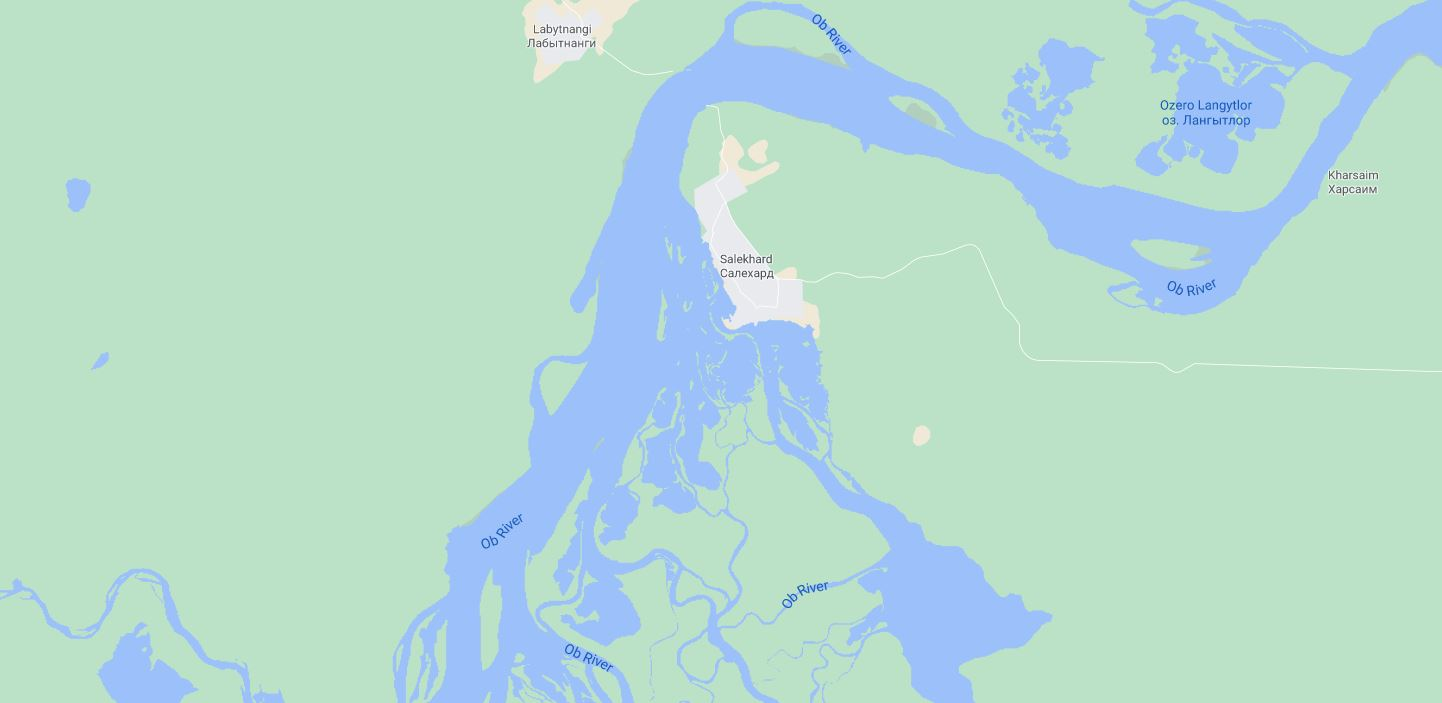
\includegraphics[width=0.9\textwidth]{salekhard} % Datei in "bilder/" bei LaTeX: eps, bei PDFLaTeX: jpg (o.ä.) 
	\caption{Station Salekhard} 
	\label{fig:Salekhard}
\end{figure}
\subsection{Water level height}
 Among the space-borne sensors, satellite altimetry can provide surface water height successively with repeat periods of 10 and 35 days. Although satellite altimetry was initially designed for oceanography, four decades of altimetry missions have provided an opportunity to study the continental hydrological cycle as well. By using the methods mentioned later, the runoff can be estimated from the satellite water level.\\\\
 Altimetry satellites basically determine the distance from the satellite to a target surface by measuring the satellite-to-surface round-trip time of a radar pulse. However, this is not the only measurement made in the process, and a lot of other information can be extracted from altimetry.\\\\
 The magnitude and shape of the echoes (or waveforms) also contain information about the characteristics of the surface which caused the reflection. The best results are obtained over the ocean, which is spatially homogeneous, and has a surface which conforms with known statistics.
 \paragraph{Envisat}
Envisat (Environmental Satellite) is a large inactive Earth-observing satellite which is still in orbit. Operated by the European Space Agency (ESA), it was the world's largest civilian Earth observation satellite. It was launched on 1 March 2002 aboard an Ariane 5 from the Guyana Space Centre in Kourou, French Guiana, into a Sun synchronous polar orbit at an altitude of $790\pm10$ km. It orbits the Earth in about 101 minutes, with a repeat cycle of 35 days. After losing contact with the satellite on 8 April 2012, ESA formally announced the end of Envisat's mission on 9 May 2012.\\\\
In working towards the global and regional objectives of the mission, numerous scientific disciplines currently use the data acquired from the different sensors on the satellite to study such things as atmospheric chemistry, ozone depletion, biological oceanography, ocean temperature and colour, wind waves, hydrology (humidity, floods), agriculture and arboriculture, natural hazards, digital elevation modelling (using interferometry), monitoring of maritime traffic, atmospheric dispersion modelling (pollution), cartography and study of snow and ice.
\paragraph{SARAL}
SARAL (Satellite with ARgos and ALtiKa) is a cooperative altimetry technology mission of Indian Space Research Organisation (ISRO) and CNES (Space Agency of France). SARAL performs altimetric measurements designed to study ocean circulation and sea surface elevation. The payloads of SARAL are The ISRO built satellite with payloads modules (ALTIKA altimeter), DORIS, Laser Retro-reflector Array (LRA) and ARGOS-3 (Advanced Research and Global Observation Satellite) data collection system provided by CNES was launched by Indian Polar Satellite Launch Vehicle rocket into the Sun-synchronous orbit (SSO). SARAL was successfully launched on 25 February 2013. It will fill the gap between Envisat and the Sentinel 3 mission of the European GMES program.
\paragraph{Sentinel-3}
Sentinel-3 is an Earth observation satellite constellation developed by the European Space Agency as part of the Copernicus Programme. The Sentinel-3 mission's main objective is to measure sea-surface topography, sea- and land-surface temperature and ocean- and land-surface colour with accuracy in support of ocean forecasting systems, and for environmental and climate monitoring. Sentinel-3 builds directly on the heritage pioneered by ERS-2 and Envisat satellites. Near-real time data will be provided for ocean forecasting, sea-ice charting, and maritime safety services on the state of the ocean surface, including surface temperature, marine ecosystems, water quality and pollution monitoring. The satellite orbit provides a 27-day repeat for the topography package, with a 4-day sub-cycle.
\clearpage
